\section{Linear Regression and Optimization \pts{10}}

\begin{questions}

\question The Summer Tanager is a lovely rose red American songbird that migrates south in the winter. Its migration occurs primarily at nighttime. You wish to study the effects of city light and city sound on the birds' migration patterns. Your ornithologist friend asks a few birder friends for help and they collect a dataset of points containing three values:
\begin{itemize}
    \item light: amount of light in area on a scale from 1-10
    \item decibels: amount of sound in decibals on a scale from 1-10
    \item birds: number of Summer Tanager songbirds observed
\end{itemize}
You build a linear regression model 
\textbf{with an intercept} to predict the number of songbirds, given the amount of light and amount of sound. 

The dataset is much larger than you expected with $N = $ 6 million training examples.

\begin{parts}

    \part[1] \textbf{True or False:} Gradient descent would be the best choice for minimizing mean squared error on this dataset because solving in closed form would be too slow with so many training examples.
    \begin{checkboxes}
     \choice True
     \choice False
    \end{checkboxes}
    \begin{soln}
    False. Closed form is linear in $N$.
    \end{soln}
    \begin{qauthor}
    Matt
    \end{qauthor}

    \part[1] How many parameters does your linear regression model have?
    \begin{checkboxes}
     \choice 1
     \choice 2
     \choice 3
     \choice 4
     \choice 10
     \choice $N$
    \end{checkboxes}
    \begin{soln}
    3
    \end{soln}
    \begin{qauthor}
    Matt
    \end{qauthor}
    
    
    \part[1] Suppose you learn that the dataset contains lots of noise due to human error in identify the birds. \textbf{True or False:} Because the dataset contains lots of noise, gradient descent could get stuck in a saddle point (i.e. flat part of the objective function with very high MSE) before reaching a global minimum. 
    \begin{checkboxes}
     \choice True
     \choice False
    \end{checkboxes}
    \begin{soln}
    False. MSE is convex, there are no flat parts except at the minimum. 
    \end{soln}
    \begin{qauthor}
    Matt
    \end{qauthor}
    
    \part[2] You sample just a dozen training examples as shown in Figure \ref{fig:linregdata}, where the label on each point is the $y$ value, number of songbirds. Describe in plain English the function $h(\mathbf{x})$ that linear regression learns by minimizing MSE. (Your description should state what the function looks like. Include sufficient detail that a friend would be able to draw a rough sketch of the function just based on your description.)
    \begin{soln}
    A plane with its highest point in the upper left corner and its lowest point in the bottom right corner. 
    \end{soln}
    \begin{qauthor}
    Matt
    \end{qauthor}
    
\end{parts}


\begin{figure}[H]
    \begin{center}
    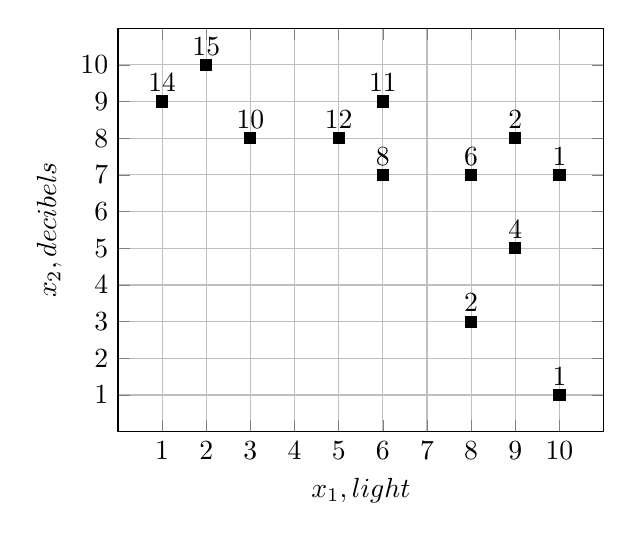
\begin{tikzpicture}
    \begin{axis}[
        scale=0.9,
        xmin=0, xmax=11, xtick={1,...,10},
        ymin=0, ymax=11, ytick={1,...,10},
        samples=50, grid=major, xlabel=$x_1\text{, light}$, ylabel=$x_2\text{, decibels}$]
        %\addplot[blue, ultra thick] (x,x*x);
        %\addplot[red,  ultra thick] (x*x,x);
        \addplot [
            scatter,
            only marks,
            point meta=explicit symbolic,
            scatter/classes={
                a={mark=square*,black},
                b={mark=triangle*,red}
            },
            nodes near coords*={$\pgfmathprintnumber[frac]\myvalue$},
            visualization depends on={\thisrow{myvalue} \as \myvalue},
        ] table [meta=label] {
            x y label myvalue
            10 1 a 1
            8 3 a 2
            9 5 a 4
            10 7 a 1
            8 7 a 6
            9 8 a 2
            6 7 a 8
            6 9 a 11
            3 8 a 10
            5 8 a 12
            1 9 a 14
            2 10 a 15
        };
    \end{axis}
    \end{tikzpicture}
    \end{center}
    \caption{}
    \label{fig:linregdata}
\end{figure}


\question Next you consider a not-so-linear variant of Linear Regression with two parameters $a$ and $b$. Given an instance $\xv = [x_1, x_2]^T$ the model predicts:
\begin{align}
    \hat{y} = h_{a,b}(\xv) = a x_1 + b x_2 + a^2 x_1
\end{align}
The model is trained to minimize mean squared error (MSE) with $J(a, b) = \frac{1}{N} \sum_{i=1}^N J^{(i)}(a,b)$ where $J^{(i)}(a,b) = (h_{a,b}(\xv^{(i)}) - y^{(i)})^2$ is the example-specific MSE.

\begin{parts}

    \part[2] What is the derivative of the example-specific MSE $J^{(i)}(a,b)$ with respect to $a$, i.e. $\frac{\partial J^{(i)}(a,b)}{\partial a}$?
    \begin{tcolorbox}[fit,height=2cm, width=15cm, blank, borderline={1pt}{-2pt}]
    %solution
    \end{tcolorbox}
    \begin{soln}
    \begin{align}
        \frac{\partial J^{(i)}(a,b)}{\partial a} 
        &= \frac{\partial}{\partial a}  ((a x_1^{(i)} + b x_2^{(i)} + a^2 x_1^{(i)}) - y^{(i)})^2 \\
        &=  2 ((a x_1^{(i)} + b x_2^{(i)} + a^2 x_1^{(i)}) - y^{(i)}) (x_1^{(i)} + 2 a x_1^{(i)}) \\
        &=  2 (h_{a,b}(\xv^{(i)}) - y^{(i)}) (x_1^{(i)} + 2 a x_1^{(i)})
    \end{align}
    \end{soln}
    \begin{qauthor}
    Matt
    \end{qauthor}
    
    \part[2] What is the derivative of the example-specific MSE $J^{(i)}(a,b)$ with respect to $b$, i.e. $\frac{\partial J^{(i)}(a,b)}{\partial b}$?
    \begin{tcolorbox}[fit,height=2cm, width=15cm, blank, borderline={1pt}{-2pt}]
    %solution
    \end{tcolorbox}
    \begin{soln}
    \begin{align}
        \frac{\partial J^{(i)}(a,b)}{\partial b} 
        &= \frac{\partial}{\partial b}  ((a x_1^{(i)} + b x_2^{(i)} + a^2 x_1^{(i)}) - y^{(i)})^2 \\
        &=  2 ((a x_1^{(i)} + b x_2^{(i)} + a^2 x_1^{(i)}) - y^{(i)}) (x_2^{(i)}) \\
        &=  2 (h_{a,b}(\xv^{(i)}) - y^{(i)}) (x_2^{(i)}) \\
    \end{align}
    \end{soln}
    \begin{qauthor}
    Matt
    \end{qauthor}
    
    \part[2] Suppose the parameters are initialized to $a = 2$ and $b = 1$. Given a dataset consisting of only one training example $(\xv = [-1, 4]^T,\, y = -3)$, what are the parameters after one epoch of gradient descent? Assume the learning rate $\gamma = 0.1$
    \begin{tcolorbox}[fit,height=1cm, width=15cm, blank, borderline={1pt}{-2pt}]
    %solution
    \end{tcolorbox}
    \begin{soln}
    \begin{align}
        & h_{a,b}(\xv) = 2(-1) + 1(4) + 2^2(-1) = -2 \\
        & dJ^{(i)}(a,b)/da = 2(-2 + 3)(-1 + 2(2)(-1)) = -10 \\
        & dJ^{(i)}(a,b)/db = 2(-2 + 3)(4) = 8 \\
        & a \rightarrow 2 - 0.1 * (-10) = 3 \\
        & b \rightarrow 1 - 0.1 * 8 = .2 
    \end{align}
    \end{soln}
    \begin{qauthor}
    Matt
    \end{qauthor}
    
    
\end{parts}


\end{questions}